\documentclass[crop,tikz]{standalone}

\usepackage{makecell}

\definecolor{alizarin}{rgb}{0.82, 0.1, 0.26}
\definecolor{airforceblue}{rgb}{0.36, 0.54, 0.66}
\definecolor{apricot}{rgb}{0.98, 0.81, 0.69}
\definecolor{blush}{rgb}{0.87, 0.36, 0.51}
\definecolor{cadmiumgreen}{rgb}{0.0, 0.42, 0.24}
\definecolor{cambridgeblue}{rgb}{0.64, 0.76, 0.68}
\definecolor{celadon}{rgb}{0.67, 0.88, 0.69}
\definecolor{chestnut}{rgb}{0.8, 0.36, 0.36}
\definecolor{harvardcrimson}{rgb}{0.79, 0.0, 0.09}
\definecolor{darkseagreen}{rgb}{0.56, 0.74, 0.56}
\definecolor{aoenglish}{rgb}{0.0, 0.5, 0.0}
\definecolor{brightube}{rgb}{0.82, 0.62, 0.91}

\usetikzlibrary{positioning}
\usetikzlibrary{matrix}
\usetikzlibrary{fit}
\usetikzlibrary{calc,decorations.pathmorphing,patterns}

\newcommand{\vvector}[1]{\tikz{\draw[#1,step=1em,fill=#1!50] (0,0)  grid (1em,4em) rectangle (0, 0);}}
\newcommand{\hvector}[1]{\tikz{\draw[#1,step=1em,fill=#1!50] (0,0)  grid (4em,1em) rectangle (0, 0);}}
\newcommand{\vvectorSmall}[1]{\tikz{\draw[#1,step=.5em,fill=#1!50] (0,0)  grid (.5em,1.5em) rectangle (0, 0);}}

\newdimen\XCoord
\newdimen\YCoord
\newdimen\XXCoord
\newdimen\YYCoord

\newcommand{\outgoing}[2]{
  \path (#1); \pgfgetlastxy{\XCoord}{\YCoord};
  \path (#2); \pgfgetlastxy{\XXCoord}{\YYCoord};
  \draw[->, line width=1pt] (\XCoord, \YCoord) -- (\XCoord, \YYCoord);
}%
\newcommand{\incoming}[2]{
  \path (#1); \pgfgetlastxy{\XCoord}{\YCoord};
  \path (#2); \pgfgetlastxy{\XXCoord}{\YYCoord};
  \draw[->, line width=1pt] (\XCoord, \YYCoord) -- (\XCoord, \YCoord);
}%


% French 
%\newcommand{\initial}{représentation \\ initiale}
%\newcommand{\final}{représentation \\ contextualisée}

% English

\newsavebox{\voc}
\sbox{\voc}{
  \begin{tabular}{|ll l ll|}
    \hline
    \multicolumn{5}{|c|}{\textbf{Vocabulaire}} \\
    \hline
    , & 1       && Rodrigue & 6 \\
    ? & 2       && dit      & 7  \\
    Chimène & 3 && cru      & 8  \\
    l'  & 4     && eût      & 9  \\
    qui & 5     &&  \\ 
    \hline
  \end{tabular}
}

\begin{document}

  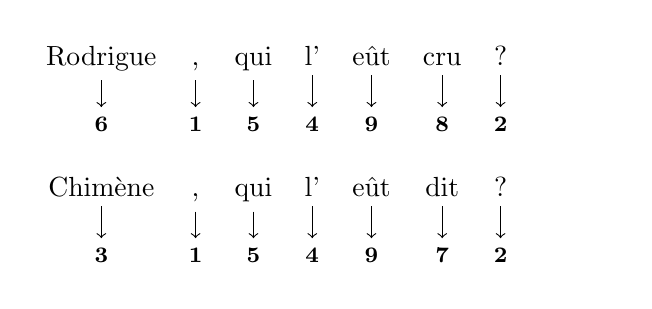
\begin{tikzpicture}[ampersand replacement=\&]
    \matrix (M) [matrix of nodes,
                 /tikz/every even row/.style={font=\footnotesize\bfseries},
                 row sep=1em,
                 column sep=.5em,]
    {
      Rodrigue \& , \& qui    \& l'    \& eût \& cru \& ?  \\
      6        \& 1 \& 5      \& 4     \& 9   \& 8   \& 2  \\
      Chimène  \& , \& qui    \& l'    \& eût \& dit \& ?  \\
      3        \& 1 \& 5      \& 4     \& 9   \& 7   \& 2 \\
    };

    \node (what) [right=of M] {\usebox{\voc}};\\

    \foreach \x in {1,2,3,4,5,6,7} {
      \draw[->] (M-1-\x) -- (M-2-\x);
    }

    \foreach \x in {1,2,3,4,5,6,7} {
      \draw[->] (M-3-\x) -- (M-4-\x);
    }

  \end{tikzpicture}

\end{document}